\documentclass[dvips, lscape]{foils}
%\documentclass[dvips, french]{slides}
\textwidth 18.5cm
\textheight 25cm 
\topmargin -1cm 
\oddsidemargin  -1cm 
\evensidemargin  -1cm

% Maths
\usepackage{amsfonts, amsmath, amssymb, url}

\newcommand{\coefbin}[2]{\left( 
    \begin{array}{c} #1 \\ #2 \end{array} 
  \right)}
\newcommand{\bbullet}{\bullet\bullet}
\newcommand{\bbbullet}{\bbullet\bullet}
\newcommand{\bbbbullet}{\bbbullet\bullet}
\newcommand{\Bcal}{\mathcal{B}}
\newcommand{\Ccal}{\mathcal{C}}
\newcommand{\Dcal}{\mathcal{D}}
\newcommand{\Ecal}{\mathcal{E}}
\newcommand{\Gcal}{\mathcal{G}}
\newcommand{\Mcal}{\mathcal{M}}
\newcommand{\Ncal}{\mathcal{N}}
\newcommand{\Pcal}{\mathcal{P}}
\newcommand{\Qcal}{\mathcal{Q}}
\newcommand{\Rcal}{\mathcal{R}}
\newcommand{\Hcal}{\mathcal{H}}
\newcommand{\Jcal}{\mathcal{J}}
\newcommand{\Lcal}{\mathcal{L}}
\newcommand{\Tcal}{\mathcal{T}}
\newcommand{\Ucal}{\mathcal{U}}
\newcommand{\Xcal}{\mathcal{X}}
\newcommand{\Zcal}{\mathcal{Z}}
\newcommand{\etabar}{\overline{\eta}}
\newcommand{\pibar}{\overline{\pi}}
\newcommand{\alphabf}{\mbox{\mathversion{bold}{$\alpha$}}}
\newcommand{\betabf}{\mbox{\mathversion{bold}{$\beta$}}}
\newcommand{\gammabf}{\mbox{\mathversion{bold}{$\gamma$}}}
\newcommand{\mubf}{\mbox{\mathversion{bold}{$\mu$}}}
\newcommand{\pibf}{\mbox{\mathversion{bold}{$\pi$}}}
\newcommand{\Pibf}{\mbox{\mathversion{bold}{$\Pi$}}}
\newcommand{\psibf}{\mbox{\mathversion{bold}{$\psi$}}}
\newcommand{\Sigmabf}{\mbox{\mathversion{bold}{$\Sigma$}}}
\newcommand{\taubf}{\mbox{\mathversion{bold}{$\tau$}}}
\newcommand{\thetabf}{\mbox{\mathversion{bold}{$\theta$}}}
\newcommand{\Abf}{{\bf A}}
\newcommand{\Ebf}{{\bf E}}
\newcommand{\Hbf}{{\bf H}}
\newcommand{\Ibf}{{\bf I}}
\newcommand{\Obf}{{\bf 0}}
\newcommand{\Sbf}{{\bf S}}
\newcommand{\mbf}{{\bf m}}
\newcommand{\ubf}{{\bf u}}
\newcommand{\vbf}{{\bf v}}
\newcommand{\xbf}{{\bf x}}
\newcommand{\Xbf}{{\bf X}}
\newcommand{\ybf}{{\bf y}}
\newcommand{\Zbf}{{\bf Z}}
\newcommand{\Esp}{{\mathbb E}}
\newcommand{\Corr}{{\mathbb C}\mbox{orr}}
\newcommand{\Nbb}{\mathbb{N}}
\newcommand{\Nm}{N(\mbf)}
\newcommand{\mum}{\mu(\mbf)}
\newcommand{\obs}{\text{obs}}
\newcommand{\ERMG}{\text{EMRG}}
\newcommand{\Ibb}{{\mathbb I}}
\newcommand{\Omegas}{\underset{s}{\Omega}}
\newcommand{\Var}{{\mathbb V}}
\newcommand{\Pro}{\mathbb{P}}
\newcommand{\Rbb}{\mathbb{R}}
\newcommand{\RX}{R_{\Xbf}}
\newcommand{\Vsf}{\mathsf{V}}
\newcommand{\Starsf}{\mathsf{*}}

% Couleur et graphiques
\usepackage{color}
\usepackage{graphics}
\usepackage{epsfig} 
\usepackage{pstcol}

% Texte
\usepackage{lscape}
\usepackage{../../../../Latex/fancyheadings, rotating, enumerate}
%\usepackage[french]{babel}
\usepackage[latin1]{inputenc}
%\definecolor{darkgreen}{cmyk}{0.5, 0, 0.5, 0.5}
%\definecolor{green}{cmyk}{0.5, 0, 0.5, 0.5}
\definecolor{orange}{cmyk}{0, 0.6, 0.8, 0}
\definecolor{jaune}{cmyk}{0, 0.5, 0.5, 0}
\newcommand{\textblue}[1]{\textcolor{blue}{#1}}
\newcommand{\textred}[1]{\textcolor{red}{#1}}
\newcommand{\textgreen}[1]{\textcolor{green}{ #1}}
\newcommand{\textlightgreen}[1]{\textcolor{green}{#1}}
%\newcommand{\textgreen}[1]{\textcolor{darkgreen}{#1}}
\newcommand{\textorange}[1]{\textcolor{orange}{#1}}
\newcommand{\textyellow}[1]{\textcolor{yellow}{#1}}
\newcommand{\emphase}[1]{\textblue{\sl #1}}
\newcommand{\refer}[1]{\textgreen{\sl #1}}

% Sections
%\newcommand{\chapter}[1]{\centerline{\LARGE \textblue{#1}}}
% \newcommand{\section}[1]{\centerline{\Large \textblue{#1}}}
% \newcommand{\subsection}[1]{\noindent{\Large \textblue{#1}}}
% \newcommand{\subsubsection}[1]{\noindent{\large \textblue{#1}}}
% \newcommand{\paragraph}[1]{\noindent {\textblue{#1}}}
% Sectionsred
\newcommand{\chapter}[1]{
  \addtocounter{chapter}{1}
  \setcounter{section}{0}
  \setcounter{subsection}{0}
  {\centerline{\LARGE \textblue{\arabic{chapter} - #1}}}
%  {\centerline{\LARGE \textblue{#1}}}
  }
\newcommand{\section}[1]{
  \addtocounter{section}{1}
  \setcounter{subsection}{0}
  {\noindent {\Large \textblue{\arabic{chapter}.\arabic{section} - #1}}}
%  {\noindent {\Large \textblue{#1}}}
  }
\newcommand{\subsection}[1]{
  \addtocounter{subsection}{1}
%   {\noindent{\large
%       \textblue{\arabic{chapter}.\arabic{section}.\arabic{subsection}
%         - #1}}}
  {\noindent{\large \textblue{#1}}}
  }
\newcommand{\paragraph}[1]{\noindent{\textblue{#1}}}

%%%%%%%%%%%%%%%%%%%%%%%%%%%%%%%%%%%%%%%%%%%%%%%%%%%%%%%%%%%%%%%%%%%%%%
%%%%%%%%%%%%%%%%%%%%%%%%%%%%%%%%%%%%%%%%%%%%%%%%%%%%%%%%%%%%%%%%%%%%%%
%%%%%%%%%%%%%%%%%%%%%%%%%%%%%%%%%%%%%%%%%%%%%%%%%%%%%%%%%%%%%%%%%%%%%%
%%%%%%%%%%%%%%%%%%%%%%%%%%%%%%%%%%%%%%%%%%%%%%%%%%%%%%%%%%%%%%%%%%%%%%
\begin{document}
%%%%%%%%%%%%%%%%%%%%%%%%%%%%%%%%%%%%%%%%%%%%%%%%%%%%%%%%%%%%%%%%%%%%%%
%%%%%%%%%%%%%%%%%%%%%%%%%%%%%%%%%%%%%%%%%%%%%%%%%%%%%%%%%%%%%%%%%%%%%%
%%%%%%%%%%%%%%%%%%%%%%%%%%%%%%%%%%%%%%%%%%%%%%%%%%%%%%%%%%%%%%%%%%%%%%
%%%%%%%%%%%%%%%%%%%%%%%%%%%%%%%%%%%%%%%%%%%%%%%%%%%%%%%%%%%%%%%%%%%%%%
\landscape
\newcounter{chapter}
\newcounter{section}
\newcounter{subsection}
\setcounter{chapter}{0}
\headrulewidth 0pt 
\pagestyle{fancy} 
\cfoot{}
\rfoot{\begin{rotate}{90}{
      \hspace{1cm} \tiny S. Robin: Mixture model for valued graphs  
      }\end{rotate}}
\rhead{\begin{rotate}{90}{
      \hspace{-.5cm} \tiny \thepage
      }\end{rotate}}

%%%%%%%%%%%%%%%%%%%%%%%%%%%%%%%%%%%%%%%%%%%%%%%%%%%%%%%%%%%%%%%%%%%%%%
%%%%%%%%%%%%%%%%%%%%%%%%%%%%%%%%%%%%%%%%%%%%%%%%%%%%%%%%%%%%%%%%%%%%%%
\begin{center}
  \textblue{\LARGE Uncovering latent structure in valued graphs:}

  \textblue{\LARGE A variational approach}
  
  ~\\~\\
  \textblue{\large \underline{S. Robin$^*$}, M. Mariadassou} \\
  ~\\~\\
  $(^*)$ UMR AgroParisTech / INRA, Paris, \\
    Math�matique et Informatique Appliqu�es \\
  \url{www.inapg.inra.fr/ens_rech/maths/} \\
  ~\\~\\
  {Statistics for Biological Sequences (SSB) group:} \\
  \url{genome.jouy.inra.fr/ssb/}
  ~\\~\\
\end{center}

\paragraph{Research report:} \\
\centerline{\url{genome.jouy.inra.fr/ssb/preprint/SSB-RR-10.valued-graphs.pdf}} 

%%%%%%%%%%%%%%%%%%%%%%%%%%%%%%%%%%%%%%%%%%%%%%%%%%%%%%%%%%%%%%%%%%%%%
%%%%%%%%%%%%%%%%%%%%%%%%%%%%%%%%%%%%%%%%%%%%%%%%%%%%%%%%%%%%%%%%%%%%%
\newpage
\chapter{Looking for structure in networks}
%%%%%%%%%%%%%%%%%%%%%%%%%%%%%%%%%%%%%%%%%%%%%%%%%%%%%%%%%%%%%%%%%%%%%
%%%%%%%%%%%%%%%%%%%%%%%%%%%%%%%%%%%%%%%%%%%%%%%%%%%%%%%%%%%%%%%%%%%%%

% %%%%%%%%%%%%%%%%%%%%%%%%%%%%%%%%%%%%%%%%%%%%%%%%%%%%%%%%%%%%%%%%%%%%%
% \bigskip
% \section{}
% %%%%%%%%%%%%%%%%%%%%%%%%%%%%%%%%%%%%%%%%%%%%%%%%%%%%%%%%%%%%%%%%%%%%%
\noindent
\begin{tabular}{cc}
  \begin{tabular}{p{12cm}}
    Networks \dots
    \begin{itemize}
    \item Arise in many fields:
      \begin{itemize}
      \item[\bf{$\rightarrow$}] Biology, Chemistry
      \item[\bf{$\rightarrow$}] Physics, Internet.
      \end{itemize}
    \item Represent an interaction pattern:
      \begin{itemize}
      \item[\bf{$\rightarrow$}] $\mathcal{O}(n^2)$ interactions
      \item[\bf{$\rightarrow$}] between $n$ elements.
      \end{itemize}
    \item Have a topology which:
      \begin{itemize}
      \item[\bf{$\rightarrow$}] reflects the structure / function
        relationship
      \end{itemize}
    \end{itemize}
  \end{tabular}
  &
  \begin{tabular}{c}
    \psfig{file=../Figures/caida2_lg(brown).ps, angle=270, width=11cm} \\
    \begin{tiny} From Barab\'asi website \end{tiny}
  \end{tabular}
\end{tabular}

%%%%%%%%%%%%%%%%%%%%%%%%%%%%%%%%%%%%%%%%%%%%%%%%%%%%%%%%%%%%%%%%%%%%%
\newpage
\paragraph{Uncovering structure in networks:} A simple example

\vspace{-2cm}
$$
\begin{tabular}{c}
  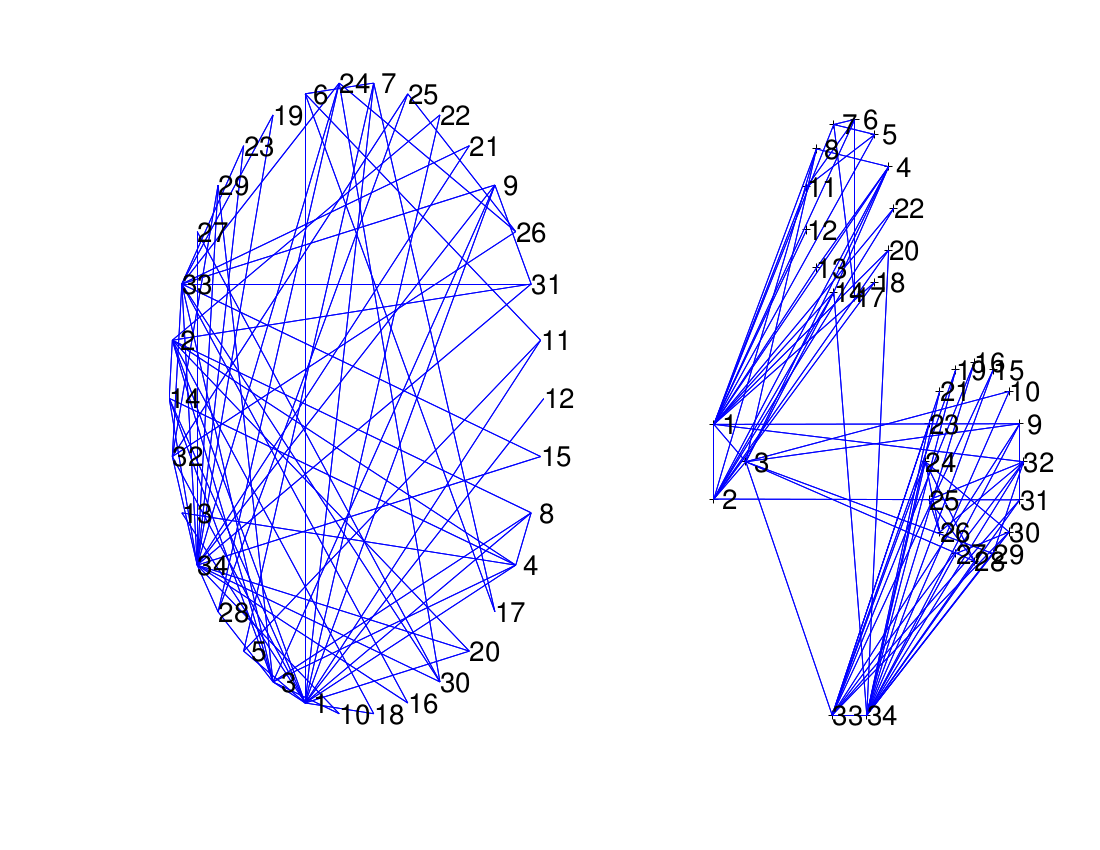
\epsfig{file = ../Figures/Karate-Graph.eps, clip=, width=7cm,
    height=20cm, angle=270}
  \\
  \epsfig{file = ../Figures/Karate-Dotplot.eps, clip=, width=7cm,
    height=20cm, angle=270}
\end{tabular}
$$


%%%%%%%%%%%%%%%%%%%%%%%%%%%%%%%%%%%%%%%%%%%%%%%%%%%%%%%%%%%%%%%%%%%%
\newpage
\section{Heterogeneity in random graphs}
%%%%%%%%%%%%%%%%%%%%%%%%%%%%%%%%%%%%%%%%%%%%%%%%%%%%%%%%%%%%%%%%%%%%%

Nodes may have different connectivity behaviour.

\paragraph{Looking for connected sub-groups:}
\begin{itemize}
\item \vspace{-0.5cm} Detection of cliques or groups of highly
  connected nodes: \refer{Gethor \& Diehl, 04} 
\item \vspace{-0.5cm} Edge betweenness: \refer{Girvan \& Newman, 02}
\item \vspace{-0.5cm} Spectral clustering: \refer{Von Luxburg \& al.,
    07}
\end{itemize}

\paragraph{Model based:}
\begin{itemize}
\item \vspace{-0.5cm} Underlying topology: \refer{Hoff \& al., 02}
  (Latent space)
\item \vspace{-0.5cm} Mixture model \refer{Nowicki \& Snijders, 01}
  (Block structure), \refer{Daudin \& al., 08} (Mixture for graphs)
\item \vspace{-0.5cm} General model for heterogeneous networks:
  \refer{Bollob\'as \ al., 07} (Topolical properties: Giant component,
  diameter, degree distribution = compound Poisson, {\it etc.}).
\item \vspace{-0.5cm} General review on random graph models:
  \refer{Pattison \& Robbins, 07}
\end{itemize}

%%%%%%%%%%%%%%%%%%%%%%%%%%%%%%%%%%%%%%%%%%%%%%%%%%%%%%%%%%%%%%%%%%%%
\newpage
\section{Inhomogeneous random graphs}
%%%%%%%%%%%%%%%%%%%%%%%%%%%%%%%%%%%%%%%%%%%%%%%%%%%%%%%%%%%%%%%%%%%%%

\paragraph{General definition for binary graphs.} (\refer{Bollob\'as \ al., 07})
\begin{itemize}
\item \vspace{-0.5cm} $n$ nodes $(i = 1 \dots n$)
\item \vspace{-0.5cm} $n(n-1)/2$ possible edges: $X_{ij} = \Ibb\{ i \sim j\}$
\item \vspace{-0.5cm} Each $i$ is characterised by a \emphase{latent
    variable} $Z_i$ sampled in some space $\Zcal$ with distribution
  $\alpha$:
  $$
  \{Z_i\}_i \mbox{ i.i.d.}, \qquad Z_i \sim \alpha
  $$
\item \vspace{-0.5cm} Edge $(i, j)$ is present with probability
  $\pi(Z_i, Z_j)$, where $\pi$ is a \emphase{kernel function}:
  $$
  \{X_{ij}\}_{i, j} \mbox{ independent given } \{Z_i\}_i, \qquad X_{ij}
  \sim \Bcal[\pi(Z_i, Z_j)].
  $$
\end{itemize}
\paragraph{Latent space:} 
$\displaystyle{
\Zcal = \Rbb^k, \qquad \pi(z, z') = \frac{\exp(a - |z-z'|)}{1 + \exp(a
  - |z-z'|)}.
}$

\paragraph{Mixture model:} 
$\displaystyle{
\Zcal = \{1, \dots, Q\}, \qquad \pi(z, z') = \pi_{q\ell} \mbox{ for } z
= q, z' = \ell.
}$

%%%%%%%%%%%%%%%%%%%%%%%%%%%%%%%%%%%%%%%%%%%%%%%%%%%%%%%%%%%%%%%%%%%%%
%%%%%%%%%%%%%%%%%%%%%%%%%%%%%%%%%%%%%%%%%%%%%%%%%%%%%%%%%%%%%%%%%%%%%
\newpage
\chapter{Mixture model for valued graphs}
%%%%%%%%%%%%%%%%%%%%%%%%%%%%%%%%%%%%%%%%%%%%%%%%%%%%%%%%%%%%%%%%%%%%%
%%%%%%%%%%%%%%%%%%%%%%%%%%%%%%%%%%%%%%%%%%%%%%%%%%%%%%%%%%%%%%%%%%%%%

\bigskip
\paragraph{Our approach}
\begin{itemize}
\item \vspace{-0.5cm} is model based: 
  $$
  \mbox{Mixture model}
  $$
\item \vspace{-0.5cm} deals with valued graphs:
  $$
  \mbox{$X_{ij} \in \{0, 1\}, \Nbb, \Rbb, \Rbb^d, {\it etc.}$}
  $$
\item \vspace{-0.5cm} and makes frequentist inference using a
  variational method :
  $$
  \mbox{Approximate maximum likelihood.}
  $$
\end{itemize}

%%%%%%%%%%%%%%%%%%%%%%%%%%%%%%%%%%%%%%%%%%%%%%%%%%%%%%%%%%%%%%%%%%%%%
\newpage
\section{Model}
%%%%%%%%%%%%%%%%%%%%%%%%%%%%%%%%%%%%%%%%%%%%%%%%%%%%%%%%%%%%%%%%%%%%%

\begin{itemize}
\item \vspace{-0.5cm} $n$ nodes $(i = 1 \dots n$);
\item \vspace{-0.5cm} each node $i$ belong to class $q$ with
  probability $\alpha_q$:
  $$
  \{Z_i\}_i \mbox{ i.i.d.}, \qquad Z_i \sim \Mcal(1; \alphabf)
  $$
  where $\alphabf = (\alpha_1, \dots \alpha_Q)$;
\item \vspace{-0.5cm} The values of the edges $\{X_{ij}\}_{i,
      j}$ are conditionally independent given the $Z_i$'s:
  $$
  (X_{ij} \;|\; Z_i = q, Z_j = \ell) \sim f_{q\ell}(\cdot).
  $$
  where $f_{q\ell}(\cdot)$ is some parametric distribution
  $f_{q\ell}(x) = f(x; \theta_{q\ell})$. \\ ~\\
\end{itemize}
We denote: $\Zbf = \{Z_i\}_i$, $\Xbf = \{X_{ij}\}_{i, j}$, $\thetabf =
\{\theta_{q\ell}\}_{q, \ell}$, $\gammabf = (\alphabf, \thetabf)$.

%%%%%%%%%%%%%%%%%%%%%%%%%%%%%%%%%%%%%%%%%%%%%%%%%%%%%%%%%%%%%%%%%%%%%
\newpage
\section{Some distributions $f_{q\ell}$}
%%%%%%%%%%%%%%%%%%%%%%%%%%%%%%%%%%%%%%%%%%%%%%%%%%%%%%%%%%%%%%%%%%%%%

\paragraph{Bernoulli $\Bcal(\pi_{ql})$.} Binary oriented or
non-oriented \emphase{interaction graphs}: \\
Relation network, protein-protein interaction, gene regulation.

\paragraph{Multinomial $\Mcal(\pibf_{ql})$.} \emphase{Labelled edges}: \\
Social networks ('friend', 'lover', colleague'), Directed graphs with
correlated edges (' ', '$\rightarrow$', '$\leftarrow$',
'$\leftrightarrow$').

\paragraph{Poisson $\Pcal(\lambda_{ql})$.} The edge value is a \emphase{count}:
\\
Number of co-publications of two authors, Number of times two species
were observed in the same place, Number of alleles shared by two
species.

\paragraph{Gaussian $\Ncal(\mu_{q\ell}, \sigma^2)$.} \emphase{Traffic
  intensity}: \\
Airport network, Electric network.

\paragraph{Linear regression.} If \emphase{covariates} $\ybf_{ij}$ are
available for each couple of nodes:
$$
X_{ij} = \ybf_{ij} \betabf_{q\ell} + E_{ij}, \qquad \{E_{ij}\}_{i, j}
\mbox{ independent, } E_{ij} \sim \Ncal(0, \sigma^2).
$$


%%%%%%%%%%%%%%%%%%%%%%%%%%%%%%%%%%%%%%%%%%%%%%%%%%%%%%%%%%%%%%%%%%%%%
%%%%%%%%%%%%%%%%%%%%%%%%%%%%%%%%%%%%%%%%%%%%%%%%%%%%%%%%%%%%%%%%%%%%%
\newpage
\chapter{Variational inference}
%%%%%%%%%%%%%%%%%%%%%%%%%%%%%%%%%%%%%%%%%%%%%%%%%%%%%%%%%%%%%%%%%%%%%
%%%%%%%%%%%%%%%%%%%%%%%%%%%%%%%%%%%%%%%%%%%%%%%%%%%%%%%%%%%%%%%%%%%%%

%%%%%%%%%%%%%%%%%%%%%%%%%%%%%%%%%%%%%%%%%%%%%%%%%%%%%%%%%%%%%%%%%%%%%
\bigskip
\section{Maximum Likelihood Inference}
%%%%%%%%%%%%%%%%%%%%%%%%%%%%%%%%%%%%%%%%%%%%%%%%%%%%%%%%%%%%%%%%%%%%%

\paragraph{Likelihoods.} The log-likelihood of the complete dataset
($\Xbf, \Zbf$) is
\begin{eqnarray*}
  \log{\Pro(\Zbf,\Xbf; \alphabf, \thetabf)} & = & \log\Pro(\Zbf; \alphabf) +
    \log{\Pro(\Xbf | \Zbf; \thetabf)} \\
  & = & \sum_i \sum_q Z_{iq}\log{\alpha_q} + \sum_{i \neq j}
  \sum_{q,\ell} Z_{iq}Z_{j\ell}\log{f_{q\ell}(X_{ij})}.
\end{eqnarray*}
The log-likelihood of the observed dataset ($\Xbf$) is
$$
\log{\Pro(\Xbf; \alphabf, \thetabf)} = \sum_{\Zbf} \log{\Pro(\Zbf,\Xbf;
  \alphabf, \thetabf)}
$$
and cannot be evaluated since $\Zbf$ may take $Q^n$ different
values. \\

\paragraph{Most popular solution:} E-M algorithm.

%%%%%%%%%%%%%%%%%%%%%%%%%%%%%%%%%%%%%%%%%%%%%%%%%%%%%%%%%%%%%%%%%%%%%
\newpage
\paragraph{E-M algorithm.} To achieve the E-step, we need to calculate
the conditional distribution of the unobserved data given the observed
ones: $\log{\Pro(\Zbf|\Xbf)}$.

\paragraph{Due to intricate dependencies} this distribution is
\emphase{intractable}:
$$
\begin{tabular}{p{11cm}p{11cm}}
  \paragraph{Dependency graph} (oriented) & \paragraph{Moral graph}
  (parents are married) \\  
  \\
  Edge $X_{ij}$ only depends on its two parents $Z_1$ and $Z_2$
  &
  Conditional on the edges, labels $Z_i$'s all depend on each others \\
                                %\\
  \hspace{-1cm}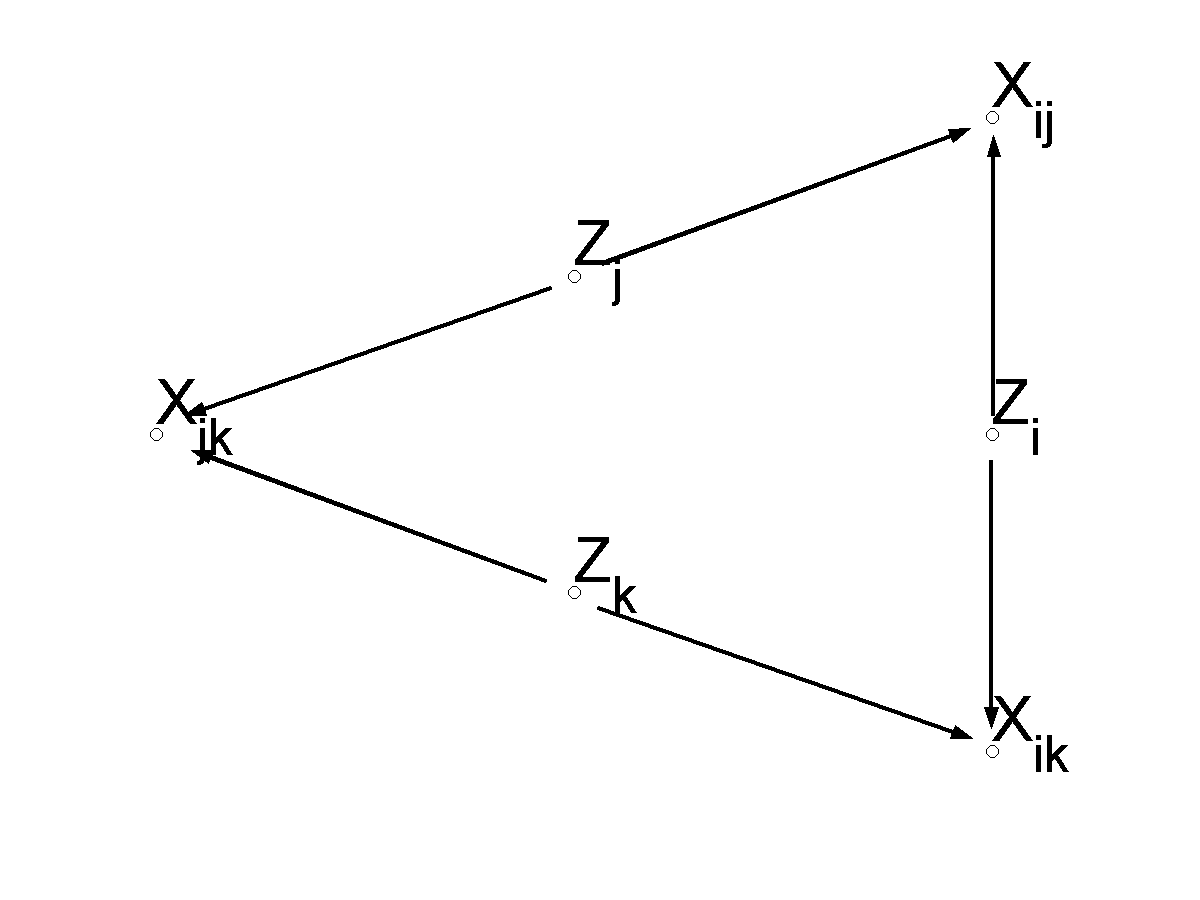
\epsfig{file = ../figures/FigNetworks-DepGraph.eps, clip=,
    angle=270, width=11cm}
  &
  \hspace{-1cm}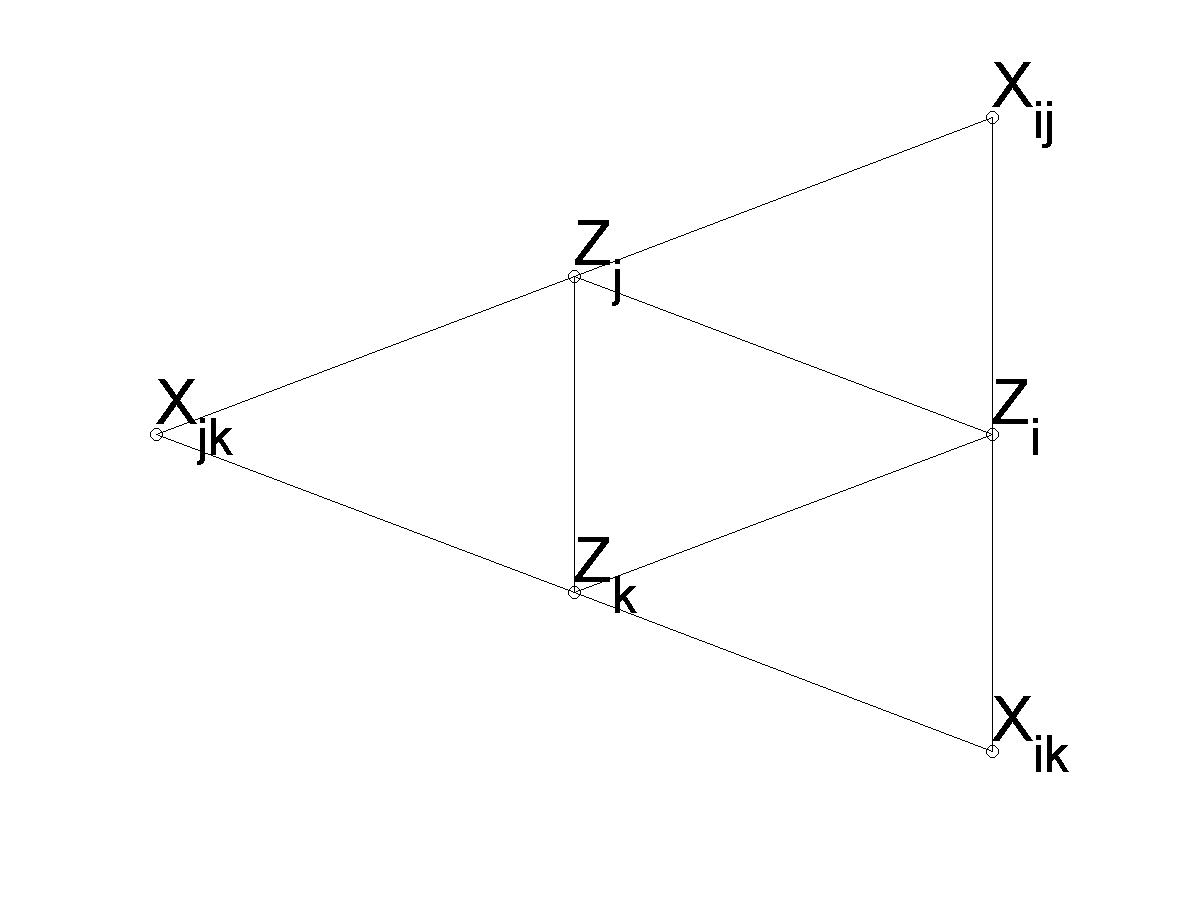
\epsfig{file = ../figures/FigNetworks-DepGraph-Moral.eps, clip=,
    angle=270, width=11cm} \\
  \multicolumn{2}{c}{\vspace{-0.5cm}$\Rightarrow$ All edges are
    actually \emphase{'neighbours'} (unlike for Bayesian networks).}
\end{tabular}
$$

%%%%%%%%%%%%%%%%%%%%%%%%%%%%%%%%%%%%%%%%%%%%%%%%%%%%%%%%%%%%%%%%%%%%%
\newpage
\section{Variational strategy}
%%%%%%%%%%%%%%%%%%%%%%%%%%%%%%%%%%%%%%%%%%%%%%%%%%%%%%%%%%%%%%%%%%%%%

\paragraph{Variational trick:} Maximise a \emphase{lower bound} of the
incomplete likelihood
$$
\Jcal(\RX,\alphabf, \thetabf) = \log{\Pro(\Xbf;\alphabf, \thetabf)} -
KL[\RX(\cdot),\Pro(\cdot|\Xbf;\alphabf, \thetabf)]
$$
where 
\begin{itemize}
\item \vspace{-0.5cm} $KL$ denotes the Kullback-Leibler divergence 
\item \vspace{-0.5cm} $\RX$ is some distribution for $\Zbf$.
\end{itemize}
Thanks to the definition of $KL$, we get for any $\RX$
(\refer{Jaakkola, 00})
\begin{eqnarray*}
  \Jcal(\RX,\alphabf, \thetabf) & = & \log{\Pro(\Xbf)} -
  \sum_{\Zbf} \log[\RX(\Zbf)] \RX(\Zbf) + \sum_{\Zbf}
  \log[P(\Zbf|\Xbf)] \RX(\Zbf) \\
  & = & \Hcal(\RX) + \sum_{\Zbf}
  \RX(\Zbf)\log{\Pro(\Xbf, \Zbf;\alphabf, \thetabf)}
\end{eqnarray*}
where $\Hcal(\RX)$ stands for the entropy of distribution $\RX$.

%%%%%%%%%%%%%%%%%%%%%%%%%%%%%%%%%%%%%%%%%%%%%%%%%%%%%%%%%%%%%%%%%%%%%
\newpage
\paragraph{Choice of $\RX$.} $\RX$ approximates the conditional
distribution $\Pro(\Zbf|\Xbf)$. We want it to be
\begin{itemize}
\item \vspace{-0.5cm} tractable (e.g. factorised):
  $$    
  \RX(\Zbf) = \prod_i h(\Zbf_i, \taubf_i)
  $$
  where $h(\cdot, \taubf)$ denotes the multinomial distribution;
\item \vspace{-0.5cm} as close to $\Pro(\Zbf|\Xbf)$ as possible:
  $$
  \widehat{\taubf} = \arg \min
  KL[\RX(\cdot),\Pro(\cdot|\Xbf;\alphabf, \thetabf)].
  $$
\end{itemize}
We get
$$
\Jcal(\RX,\alphabf, \thetabf) = - \sum_i \sum_q \tau_{iq} \log{\tau_{iq}} +
\sum_i \sum_q \tau_{iq} \log{\alpha_q} + \sum_{i \neq j} \sum_{q,\ell}
\tau_{iq} \tau_{j\ell} \log{f_{q\ell}(X_{ij})}.
$$
The $\tau_i$'s are interpreted as \emphase{approximate posterior
  probabilities $\Pro\{Z_i = q | \Xbf\}$};

%%%%%%%%%%%%%%%%%%%%%%%%%%%%%%%%%%%%%%%%%%%%%%%%%%%%%%%%%%%%%%%%%%%%%
\newpage
\section{Estimation algorithm}
%%%%%%%%%%%%%%%%%%%%%%%%%%%%%%%%%%%%%%%%%%%%%%%%%%%%%%%%%%%%%%%%%%%%%

The optimisation of $\Jcal(\RX,\alphabf, \thetabf)$ is achieved via two
alternative steps.

\paragraph{M-step:} Maximises $\Jcal(\RX,\alphabf, \thetabf)$ w.r.t. $\alphabf, \thetabf =
(\alphabf, \thetabf)$ given $\taubf$. We get
$$
\widehat{\alpha}_q = \frac1n \sum_i \tau_{iq}, \qquad
\widehat{\theta}_{q\ell} = \arg\underset{\theta_{q\ell}}{\max} \sum_{i
  \neq j} \tau_{iq}\tau_{j\ell}\log{f(X_{ij}; \theta_{q\ell})}.
$$

\paragraph{Fix point relation.} Find the optimal $\taubf$ given
$(\alphabf, \thetabf)$. We end up with a fix point relation.
\begin{itemize}
\item \vspace{-0.5cm} Oriented graphs:
  $$
  \log \widehat{\tau}_{iq} = \mbox{cst} + \log \alpha_q + \sum_{j
    \neq i} \sum_{\ell} \widehat{\tau}_{j\ell} \left[\log
    f(X_{ij}; \theta_{q\ell}) \log f(X_{ji}; \theta_{\ell q})\right].
  $$
\item \vspace{-0.5cm} Non-oriented graphs:
  $$
  \log \widehat{\tau}_{iq} = \mbox{cst} + \log \alpha_q + \sum_{j
    \neq i} \sum_{\ell} \widehat{\tau}_{j\ell} \log f(X_{ij};
  \theta_{q\ell}).
  $$
\end{itemize}


%%%%%%%%%%%%%%%%%%%%%%%%%%%%%%%%%%%%%%%%%%%%%%%%%%%%%%%%%%%%%%%%%%%%%
\newpage
\section{Model selection}
%%%%%%%%%%%%%%%%%%%%%%%%%%%%%%%%%%%%%%%%%%%%%%%%%%%%%%%%%%%%%%%%%%%%%

\paragraph{Penalised likelihood.} Standard criteria, such as BIC or
AIC are based on the log-likelihood of observed data $\log
\Pro(\Xbf)$, so they can not be used here.

\paragraph{Integrated Classification Likelihood (ICL).} The ICL
criterion (\refer{Biernacki \& al., 00}) is an approximation of the
complete-data integrated log-likelihood:
$$
\log \Pro(\Xbf, \Zbf| m_Q) = \int \log \Pro(\Xbf, \Zbf |
\gammabf,m_Q) g(\gammabf|m_Q) d\gammabf,
$$
where $\log \Pro(\Xbf, \Zbf | \gammabf,m_Q)$ is the log-likelihood
of model $m_Q$ with $Q$ classes.

We get
$$
ICL(m_Q) = \underset{\gammabf}{\max} \log \Pro(\Xbf,
\widehat{\Zbf} |\gammabf, m_Q) - \frac{1}{2} \left\{ P_Q \log
  [n(n-1)] - (Q-1) \log(n) \right\}.
$$
where $P_Q$ denotes the number of parameters in $\thetabf$ and
$\widehat{\Zbf}$ can be replaced by $\widehat{\taubf}$ or by the
Maximum A posteriori (MAP) prediction of $\Zbf$.


%%%%%%%%%%%%%%%%%%%%%%%%%%%%%%%%%%%%%%%%%%%%%%%%%%%%%%%%%%%%%%%%%%%%%
%%%%%%%%%%%%%%%%%%%%%%%%%%%%%%%%%%%%%%%%%%%%%%%%%%%%%%%%%%%%%%%%%%%%%
\newpage
\chapter{Applications}
%%%%%%%%%%%%%%%%%%%%%%%%%%%%%%%%%%%%%%%%%%%%%%%%%%%%%%%%%%%%%%%%%%%%%
%%%%%%%%%%%%%%%%%%%%%%%%%%%%%%%%%%%%%%%%%%%%%%%%%%%%%%%%%%%%%%%%%%%%%

%%%%%%%%%%%%%%%%%%%%%%%%%%%%%%%%%%%%%%%%%%%%%%%%%%%%%%%%%%%%%%%%%%%%%
\bigskip
\section{Metabolic network of {\sl E. coli}}
%%%%%%%%%%%%%%%%%%%%%%%%%%%%%%%%%%%%%%%%%%%%%%%%%%%%%%%%%%%%%%%%%%%%%

\paragraph{Dataset.}
\begin{itemize}
\item \vspace{-0.5cm} The network is made of 605 reaction (nodes) and
  1782 edges (\refer{V Lacroix \& M.-F. Sagot, INRIA}).
\item \vspace{-0.5cm} Reactions $i$ and $j$ are connected if the
  compound of $i$ is the substrate of $j$.
\item \vspace{-0.5cm} Because most reactions are reversible, the
  network is not oriented.
\item \vspace{-0.5cm} The only information about edges is terms of
  presence/absence.
\end{itemize}
\paragraph{Results} 
\begin{itemize}
\item \vspace{-0.5cm} The ICL criterion applied to a mixture with
  Bernoulli edge values select $\widehat{Q} = 21$ classes.
    \item \vspace{-0.5cm} Groups 1 to 20 gather reactions involving
      all the \emphase{same compound} either as a substrate or as a
      product.
    \item \vspace{-0.5cm} A compound (chorismate, pyruvate,
      ATP,\emph{etc}) can be associated to each group.
\end{itemize}


%%%%%%%%%%%%%%%%%%%%%%%%%%%%%%%%%%%%%%%%%%%%%%%%%%%%%%%%%%%%%%%%%%%%%
\newpage
\paragraph{Dot-plot representation.} \\
\begin{tabular}{cc}
  \begin{tabular}{p{12cm}}
    \begin{itemize}
    \item Classes 1 and 16 constitute a \emphase{single clique}
      corresponding to a single compound (pyruvate),
    \item They are split into two classes because they
      \emphase{interact differently with classes 7} (CO2) and 10
      (AcetylCoA)
    \item Connectivity matrix (sample): 
      $$
      \begin{array}{c|cccc}
        q, \ell & 1 & 7 & 10 & 16 \\
        \hline
        1  & \textcolor{red}{1.0} & & & \\
        7  & \textcolor{green}{.11} & .65 & &  \\
        10 & \textcolor{green}{.43} & & .67 & \\
        16 & \textcolor{red}{1.0} & \textcolor{yellow}{.01} &
        \textcolor{yellow}{\epsilon} & \textcolor{red}{1.0}
      \end{array}
      $$
    \end{itemize}    
  \end{tabular}
  &
  \begin{tabular}{c}
    \epsfig{file = ../Figures/Ecoli-Complet-ERMG-Ward-Q21_class3.ps,
     height=12cm, width=12cm, clip=, angle=90, bbllx=33, bblly=64,
    bburx=565, bbury=389} \\
      Adjacency matrix \\
      (zoom on the 20 first classe)
   \end{tabular}
\end{tabular}

%%%%%%%%%%%%%%%%%%%%%%%%%%%%%%%%%%%%%%%%%%%%%%%%%%%%%%%%%%%%%%%%%%%%%
\subsection{}

%%%%%%%%%%%%%%%%%%%%%%%%%%%%%%%%%%%%%%%%%%%%%%%%%%%%%%%%%%%%%%%%%%%%%
\newpage
\section{Gene regulations in {\sl A. Thaliana}}
%%%%%%%%%%%%%%%%%%%%%%%%%%%%%%%%%%%%%%%%%%%%%%%%%%%%%%%%%%%%%%%%%%%%%

\paragraph{Dataset.} \emphase{Partial correlations} between the expression
levels of 800 genes in various conditions (\refer{Opgen-Rhein \&
  Strimmer, 06}). \\
~\\
\begin{tabular}{cc}
  \hspace{-1cm}
  \begin{tabular}{p{12cm}}
    \paragraph{Dot-plot.} Dot size = absolute correlation, Color =
    sign (\textred{$-$}, \textblue{$+$}). \\
    ~\\
    \paragraph{Results.} 
    \begin{itemize}
    \item \vspace{-0.5cm} Using a Gaussian model, we get $\widehat{Q}
      = 7$ classes.
    \item \vspace{-0.5cm} Groups are made of positively correlated
      genes. 
    \item \vspace{-0.5cm} Between group correlations are weaker than
      within-group correlation and have different signs (see classes
      3/4 with class 7).
    \item \vspace{-0.5cm} Total computational time for $Q=1..15$
      classes on a standard PC: 1h.
    \end{itemize}
  \end{tabular}
  &
  \begin{tabular}{c}
    \hspace{-1cm}
    \epsfig{file = ../Figures/GauHo_Q7_dotplot.eps, width=13cm,
    height=13cm, clip=}
  \end{tabular}
\end{tabular}

%%%%%%%%%%%%%%%%%%%%%%%%%%%%%%%%%%%%%%%%%%%%%%%%%%%%%%%%%%%%%%%%%%%%%
\newpage
\section{Fungus - Tree interactions}
%%%%%%%%%%%%%%%%%%%%%%%%%%%%%%%%%%%%%%%%%%%%%%%%%%%%%%%%%%%%%%%%%%%%%

\paragraph{Dataset.} Interactions between 154 fungi and 51
trees European species. Fungus $f$ is connected to tree $t$ if it has
been collected on it (\refer{Data from C. Vacher, INRA}).

\paragraph{Projected graphs.} For each species we define the projected
graph:
$$
\begin{array}{lrcl}
  \mbox{for trees} \quad & X_{tt'} & = & \mbox{Number of common
  fungi,} \\ 
\\
  \mbox{for fungi} \quad & X_{ff'} & = & \mbox{Number of common trees.}
\end{array}  
$$

\paragraph{Poisson model.} For both species, we assume that the
intensities have Poisson distributions: $X
\sim\Pcal(\lambda_{q\ell})$.

\paragraph{Number of classes.} The ICL criterion selects 
\begin{itemize}
\item \vspace{-0.5cm} 5 classes for trees
\item \vspace{-0.5cm} and 6 classes for fungi.
\end{itemize}



%%%%%%%%%%%%%%%%%%%%%%%%%%%%%%%%%%%%%%%%%%%%%%%%%%%%%%%%%%%%%%%%%%%%%
\newpage
\noindent
\begin{tabular}{cc}
  \begin{tabular}{p{11cm}}
    \subsection{Fungus network}
    \\ 
    \epsfig{file = ../Figures/Fungus_Poiss_Q6_dotplot.eps,
      width=12cm, height=12cm, clip=} \\
    \begin{itemize}
    \item \vspace{-0.5cm} A group of generalist fungi is detected.
    \item \vspace{-0.5cm} Others are more specific.
    \end{itemize}
  \end{tabular}
  &
  \begin{tabular}{p{11cm}}
    \subsection{Tree network}
    \\
    \epsfig{file = ../Figures/Tree_Poiss_Q5_dotplot.eps,
      width=8cm, height=8cm, clip=}
    \\ 
    \begin{itemize}
    \item \vspace{-0.5cm} Trees are mainly clustered according to
      the number of fungi they host.
    \item \vspace{-0.5cm} Tree groups are less contrasted.
    \end{itemize}
    \\ \\ \\ \\ 
  \end{tabular}
\end{tabular}

%%%%%%%%%%%%%%%%%%%%%%%%%%%%%%%%%%%%%%%%%%%%%%%%%%%%%%%%%%%%%%%%%%%%%
\newpage
\subsection{Crossed clusterings}

%\bigskip
\noindent
\begin{tabular}{cc}
  \begin{tabular}{p{16cm}}
    The comparison of the two clusterings exhibits \emphase{specific
    correspondences} between groups of fungi (rows) and trees (columns). \\
    \\ \\
    \paragraph{Work in progress.} Compare these groups according to
    their phyla, the time of their introduction in Europe, {\it
    etc.}. \\
    \\ \\
    \paragraph{Biclustering.} A direct clustering could be performed
    on the interaction matrix Fungi $\times$ Tree. The method
    proposed by \refer{Govaert \& Nadif (05)} also relies on a
    variational approach. \\ \\
  \end{tabular}
  &
  \begin{tabular}{p{10cm}}
    \epsfig{file = ../Figures/CompCluster_QF6_QT5.eps,
    width=7cm, height=15cm, clip=}
  \end{tabular}
\end{tabular}





%%%%%%%%%%%%%%%%%%%%%%%%%%%%%%%%%%%%%%%%%%%%%%%%%%%%%%%%%%%%%%%%%%%%%
%%%%%%%%%%%%%%%%%%%%%%%%%%%%%%%%%%%%%%%%%%%%%%%%%%%%%%%%%%%%%%%%%%%%%
\newpage
\chapter{Discussion}
%%%%%%%%%%%%%%%%%%%%%%%%%%%%%%%%%%%%%%%%%%%%%%%%%%%%%%%%%%%%%%%%%%%%%
%%%%%%%%%%%%%%%%%%%%%%%%%%%%%%%%%%%%%%%%%%%%%%%%%%%%%%%%%%%%%%%%%%%%%

%%%%%%%%%%%%%%%%%%%%%%%%%%%%%%%%%%%%%%%%%%%%%%%%%%%%%%%%%%%%%%%%%%%%%
\subsection{Inference for heterogeneous valued graphs}

\begin{itemize}
\item \vspace{-0.5cm} Mixture models constitutes a natural way to
  describe heterogeneity in a network.
\item \vspace{-0.5cm} The variational approach is a general and
  efficient alternative to MCMC algorithms.
\end{itemize}

%%%%%%%%%%%%%%%%%%%%%%%%%%%%%%%%%%%%%%%%%%%%%%%%%%%%%%%%%%%%%%%%%%%%%
\subsection{Simulation of 'realistic' networks}

\begin{itemize}
\item \vspace{-0.5cm} 'Realistic' heterogeneous networks can be
  simulated according to mixture models with given parameters.
\item \vspace{-0.5cm} The \emphase{Expected Degree Distribution (EDD)}
  model (\refer{Park \& Newman, 03}, \refer{Chung \& Lu, 02}) is
  another special case of heterogeneous binary network:
  \begin{itemize} 
  \item For each node $i$, draw its \emphase{expected degree $D_i$} in
    the empirical degree distribution $F$ of a given network.
    %: $\{D_i\} \mbox{ i.i.d. }  \sim F$.
  \item For each couple of nodes $(i, j)$, the edge \emphase{$i \sim
      j$ exists with probability $D_i D_j/K$}.
    %: $(X_{ij} |D_i, D_j) \sim \Bcal(D_i D_j /K)$.
  \end{itemize}
\end{itemize}

%%%%%%%%%%%%%%%%%%%%%%%%%%%%%%%%%%%%%%%%%%%%%%%%%%%%%%%%%%%%%%%%%%%%%
\newpage
\subsection{Mixture model as a null model for heterogeneous networks}

\noindent
\begin{tabular}{cc}
  \begin{tabular}{p{15cm}}
    \paragraph{Looking for over-represented motifs in {\sl E. coli}
    transcriptional network.} \\
    \\
    \paragraph{Strategy proposed by \refer{\sl Shen-Orr \& al, 02}.} 
    \begin{enumerate}
    \item Count the number of occurrences $N_{\obs}(\mbf)$;
    \item Resample a \textblue{large number of random networks}
      similar to {\sl E.coli}'s one (using the edge swapping
      algorithm);
    \item Estimate $\Esp \Nm$ and $\Var \Nm$;
%     \item Calculate a $Z$-score: 
%       $Z = (N_{\obs}(\mbf) - \Esp \Nm)/ \sqrt{\Var \Nm}$;
    \item \textblue{Derive a $p$-value} implicitly based on a Gaussian
      approximation. 
    \end{enumerate}
  \end{tabular}
  &
  \begin{tabular}{c}
    \epsfig{file=../FIGURES/RegulationMotifs.ps, bbllx=82, bblly=89,
    bburx=289, bbury=600, clip=, height=16cm}
  \end{tabular}
\end{tabular}

%%%%%%%%%%%%%%%%%%%%%%%%%%%%%%%%%%%%%%%%%%%%%%%%%%%%%%%%%%%%%%%%%%%%%
\newpage
\subsection{Direct computation using heterogenous models}

\noindent \hspace{-1cm}
\begin{tabular}{cc}
  \begin{tabular}{p{11cm}}
    \paragraph{Exact moments.} For several heterogeneous models
    (mixture, EDD), we can get the exact formula for the mean $\Esp N$
    and variance $\Var N$ of the count (\refer{Picard \& al., 07}). \\
    \\ \\
    \paragraph{Distribution.} Based on theoretical results (Erd�s)
    and an analogy with sequence motifs, we fit a \emphase{compound
    Poisson} distribution to derive a $p$-value. \\ \\
  \end{tabular}
  &
  \begin{tabular}{p{10cm}}
    {\small \hspace{-1cm}
    \begin{tabular}{crrrr}
      Motif & $N_{\obs}(\mbf)$ & $\lambda$ & $\displaystyle{\frac1{(1-a)}}$ & $p$-value  \\
      \hline
      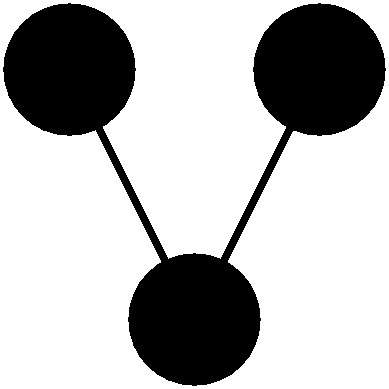
\epsfig{file = ../figures/Vmotif.eps, width=1cm, clip=} & 14\,113 & 25.5 & 514.9 & 3.36$\,10^{-1}$ \\
      \epsfig{file = ../figures/triangle.eps, width=1cm, clip=} & 75 & 10.4 & 6.2 & 2.87$\,10^{-1}$ \\
      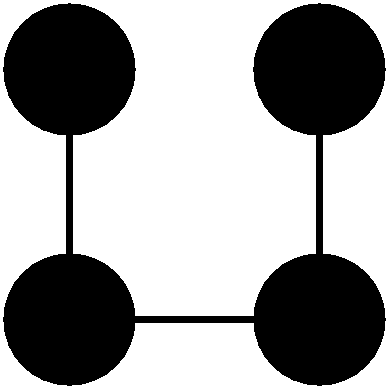
\epsfig{file = ../figures/chainmotif.eps, width=1cm, clip=} & 98\,697 & 11.9 & 7\,543.2 & 3.46$\,10^{-1}$ \\
      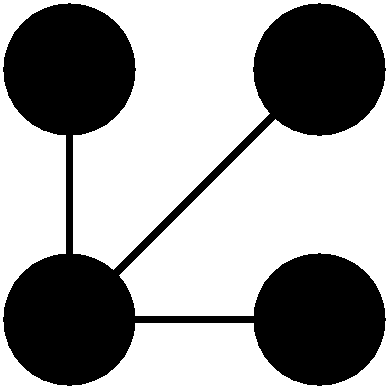
\epsfig{file = ../figures/starmotif.eps, width=1cm, clip=} & 112\,490 & 11.4 & 7\,812.0 & 1.85$\,10^{-1}$ \\
      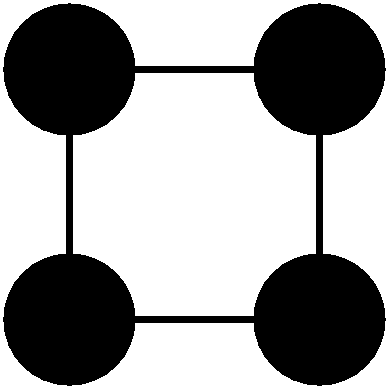
\epsfig{file = ../figures/squaremotif.eps, width=1cm, clip=} & 1\,058 & 5.9 & 82.9 & \emphase{9.34$\,10^{-3}$} \\
      \epsfig{file = ../figures/whisk.eps, width=1cm, clip=} & 3\,535 & 6.4 & 428.7 & 2.22$\,10^{-1}$ \\
      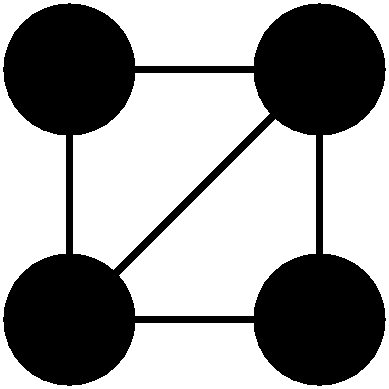
\epsfig{file = ../figures/halfclique.eps, width=1cm, clip=} & 79 & 2.9 & 11.5 & \emphase{2.56$\,10^{-2}$} \\
      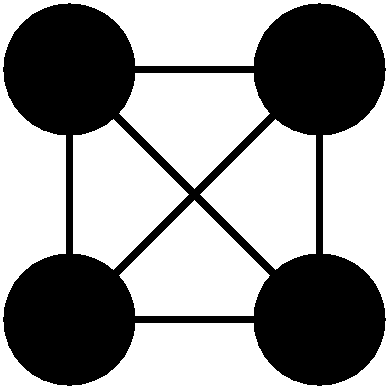
\epsfig{file = ../figures/clique.eps, width=1cm, clip=} & 0 & 0.1 & 1.1 & 1.00 \\
    \end{tabular}
    }
  \end{tabular}
\end{tabular}

\paragraph{Results for \emphase{E. coli}'s network.} 2 motifs
appear to be unexpectedly frequent. \\
\\
According to the permutation-based strategy, all of them are
significantly over-represented!


%%%%%%%%%%%%%%%%%%%%%%%%%%%%%%%%%%%%%%%%%%%%%%%%%%%%%%%%%%%%%%%%%%%%%%%%
%%%%%%%%%%%%%%%%%%%%%%%%%%%%%%%%%%%%%%%%%%%%%%%%%%%%%%%%%%%%%%%%%%%%%%%%
%%%%%%%%%%%%%%%%%%%%%%%%%%%%%%%%%%%%%%%%%%%%%%%%%%%%%%%%%%%%%%%%%%%%%%%%
%%%%%%%%%%%%%%%%%%%%%%%%%%%%%%%%%%%%%%%%%%%%%%%%%%%%%%%%%%%%%%%%%%%%%%%%
\end{document}
%%%%%%%%%%%%%%%%%%%%%%%%%%%%%%%%%%%%%%%%%%%%%%%%%%%%%%%%%%%%%%%%%%%%%%%%
%%%%%%%%%%%%%%%%%%%%%%%%%%%%%%%%%%%%%%%%%%%%%%%%%%%%%%%%%%%%%%%%%%%%%%%%
%%%%%%%%%%%%%%%%%%%%%%%%%%%%%%%%%%%%%%%%%%%%%%%%%%%%%%%%%%%%%%%%%%%%%%%%
%%%%%%%%%%%%%%%%%%%%%%%%%%%%%%%%%%%%%%%%%%%%%%%%%%%%%%%%%%%%%%%%%%%%%%%%

\noindent
\begin{tabular}{cc}
  \begin{tabular}{p{10cm}}
  \end{tabular}
  &
  \begin{tabular}{p{10cm}}
  \end{tabular}
\end{tabular}

\begin{itemize}
\item \vspace{-0.5cm} 
\item \vspace{-0.5cm} 
\item \vspace{-0.5cm} 
\end{itemize}

%%%%%%%%%%%%%%%%%%%%%%%%%%%%%%%%%%%%%%%%%%%%%%%%%%%%%%%%%%%%%%%%%%%%%
\newpage
\subsection{Significance of motifs of size 3 and 4}

2 motifs appear to be unexpectedly frequent.
$$
\begin{tabular}{crrrrrr}
 Motif & $N_{\obs}(\mbf)$ & $\Esp_{\ERMG}(N)$ & $\sigma_{\ERMG}(N)$ &
 $\lambda$ & $1/(1-a)$ & $p$-value  \\

 \hline
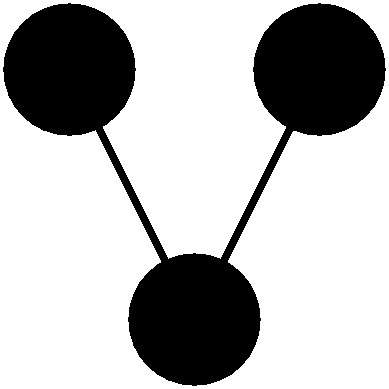
\epsfig{file = ../figures/Vmotif.eps, width=1cm, clip=} & 14\,113 & 13\,118 & 2\,599 & 25.5 & 514.9 & 3.36$\,10^{-1}$ \\
\epsfig{file = ../figures/triangle.eps, width=1cm, clip=} & 75 & 64.4 & 20 & 10.4 & 6.2 & 2.87$\,10^{-1}$ \\
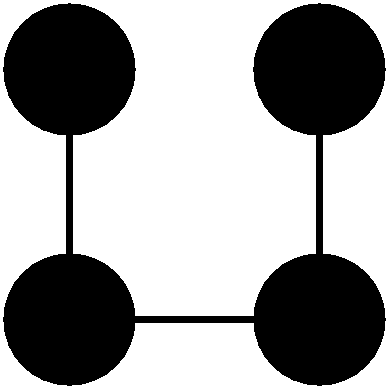
\epsfig{file = ../figures/chainmotif.eps, width=1cm, clip=} & 98\,697 & 90\,059 & 26\,064 & 11.9 & 7\,543.2 & 3.46$\,10^{-1}$ \\
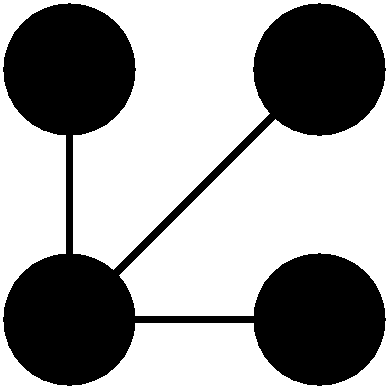
\epsfig{file = ../figures/starmotif.eps, width=1cm, clip=} & 112\,490 & 89\,372 & 26\,423 & 11.4 & 7\,812.0 & 1.85$\,10^{-1}$ \\
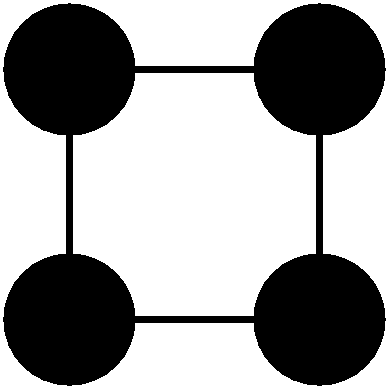
\epsfig{file = ../figures/squaremotif.eps, width=1cm, clip=} & 1\,058 & 492 & 202 & 5.9 & 82.9 & \emphase{9.34$\,10^{-3}$} \\
\epsfig{file = ../figures/whisk.eps, width=1cm, clip=} & 3\,535 & 2\,756 & 1\,087 & 6.4 & 428.7 & 2.22$\,10^{-1}$ \\
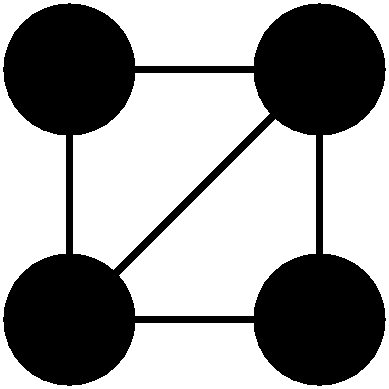
\epsfig{file = ../figures/halfclique.eps, width=1cm, clip=} & 79 &
 33.2 & 19.5 & 2.9 & 11.5 & \emphase{2.56$\,10^{-2}$} \\
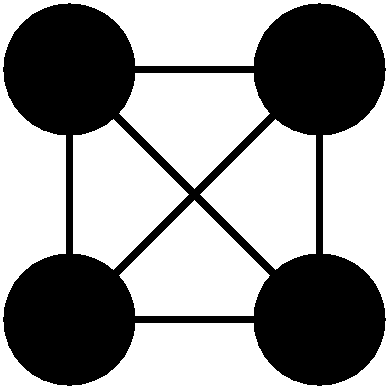
\epsfig{file = ../figures/clique.eps, width=1cm, clip=} & 0 & 0.165 & 0.432 & 0.1 & 1.1 & 1.00 \\
\end{tabular}
$$
\paragraph{Mean clump size.} $\Esp V = 1/(1-a)$.

